\section{Introduction}

Dans un contexte technologique en constante évolution, marqué par une forte concurrence et une accélération des cycles de développement, l’importance des concepts que nous avons mis en œuvre est devenue capitale. L’automatisation, qui était autrefois perçue comme un avantage optionnel, s’impose désormais comme une nécessité incontournable pour garantir la fiabilité, la sécurité et la rapidité des processus.

\section{Présentation de l'organisme d'accueil}

Oneex est une entreprise française basée à Clermont-Ferrand, avec un établissement secondaire à Paris. Elle est spécialisée dans la conception et le développement de solutions logicielles et matérielles dédiées à la vérification d’identité et à l’analyse documentaire. Grâce à des technologies avancées telles que l’intelligence artificielle et des capteurs avancés tel que les lecteurs NFC , infrarouge , hyper resolution pour une analyse approfondie des documents , qui n'est autrement pas possible a l'oeil nu, Oneex propose des solutions innovantes pour lutter contre la fraude documentaire.

\subsection{Historique de l’entreprise}

\begin{itemize}
	\item \textbf{Création de la société (2017)}  
	      Le concept Oneex est né de l’initiative de son fondateur, confronté à la problématique de l’analyse des documents d’identité. N’ayant trouvé aucune solution souveraine respectant les contraintes réglementaires sur les données personnelles, il a décidé de créer et de développer Oneex.
	      
	\item \textbf{Recherche et développement (2018-2020)}  
	      Pendant deux années, l’entreprise s’est consacrée à la recherche et au développement. Le logiciel ScanApp a ainsi été créé pour reproduire la vision humaine grâce à une intelligence artificielle capable d’analyser avec précision le pays, le format et les spécificités techniques d’un document.
	      
	\item \textbf{Déploiement de la solution Desktop (2020)}  
	      Forte de ce développement, Oneex a lancé une offre complète associant hardware et software, donnant naissance à la solution Desktop.
	      
	\item \textbf{Reconnaissance et impact (2021-2023)}  
	      L’entreprise a rapidement acquis une reconnaissance dans son domaine, obtenant des distinctions et certifications de la part de leaders de l’industrie. Elle poursuit aujourd’hui sa croissance à l’international.
	      
	\item \textbf{Percées technologiques et évolution (2023-2024)}  
	      Oneex a enrichi ses produits de nouvelles fonctionnalités, notamment le monitoring à distance, l’accès à des statistiques détaillées, la gestion autonome du parc matériel et un accompagnement expert en fraude documentaire. Après une levée de fonds importante en 2024, l’entreprise développe de nouveaux produits pour renforcer son positionnement en tant que leader de l’analyse documentaire.
\end{itemize}

% En 2025, François-Xavier Hauet, mon tuteur de stage, a rejoint l’entreprise en tant que Directeur Général. Fort d’une carrière de haut fonctionnaire et d’une expertise reconnue dans la transformation numérique, notamment à la Présidence de la République, il apporte à Oneex une vision stratégique et opérationnelle précieuse. Sous son impulsion, l’entreprise engage le développement de la nouvelle génération de ses solutions.

\subsection{Domaine d'activité}

Oneex propose des solutions transversales adaptées à de nombreux secteurs, notamment la santé, les banques, la sécurité et le contrôle d’accès, la location de véhicules, ainsi que les aéroports et compagnies aériennes. L’entreprise se distingue par son application \emph{Oneex Cloud}, une plateforme qui offre un contrôle centralisé et un suivi avancé des vérifications d’identité. 

Voici quelques fonctionnalités clés :

\begin{itemize}
	\item \textbf{Suivi des documents scannés} : historique complet, résultats détaillés et traçabilité optimale.
	\item \textbf{Demande d’expertise} : sollicitation d’experts pour garantir des analyses approfondies et fiables.
	\item \textbf{Statistiques avancées} : exploitation des tendances de la fraude pour optimiser la gestion des incidents.
\end{itemize}

Ces solutions permettent aux entreprises de contrôler efficacement les accès, de réduire les fraudes et de fluidifier les processus d’intégration dans le respect des réglementations RGPD.

\subsection{Organisation interne}

La direction et les équipes de Oneex rassemblent des profils pluridisciplinaires aux parcours variés :

\begin{description}
	\item[Alexandre Casagrande] Fondateur et Président Directeur Général. Après 12 ans au sein du Ministère des Armées et plusieurs années dans la sûreté de grands groupes, il a fondé Oneex avec la volonté de développer une solution souveraine et innovante.
	  
	\item[François-Xavier Hauet] Directeur Général. Ancien haut fonctionnaire, il a piloté la transformation numérique du Centre Interministériel de Crise puis de la Présidence de la République avant de rejoindre Oneex en 2025.
	  
	\item[Julien Otal] CTO. Développeur spécialisé dans le multiplateforme, il possède une solide expérience dans la sécurisation de systèmes critiques et la traçabilité des flux.
	  
	\item[Xavier Matton] Directeur des Opérations. Ingénieur et ancien officier au Ministère de l’Intérieur, il est expert en contrôle des flux et lutte contre la fraude documentaire.
	  
	%\item[Damien Lazardeux] Architecte Logiciels. Spécialiste des technologies .NET, il conçoit les systèmes logiciels de détection des faux papiers.
	  
	\item[Sébastien Kowalczuk] Directeur des Opérations Sud-Ouest. Ancien enquêteur en contre-ingérence économique, il apporte une expertise forte en sécurité des données sensibles.
\end{description}

% \begin{figure}[ht]
%     \centering
%     \begin{tikzpicture}[
%         sibling distance=25mm,
%         level distance=20mm,
%         edge from parent/.style={draw,-},
%         every node/.style={
%             draw,
%             fill=blue!80,
%             rectangle,
%             text=white,
%             align=center,
%             font=\sffamily
%         }
%     ]
%     \node {PRÉSIDENT \\ DIRECTEUR \\ GÉNÉRAL}
%         child {node {DIRECTEUR \\ GÉNÉRAL}
%             child {node {RESSOURCES \\ HUMAINES}}
%             child {node {DIRECTION DES \\ OPÉRATIONS}}
%             child {node {DIRECTION \\ TECHNIQUE}
%                 child {node {Mahdi}}
%             }
%             child {node {SÉCURITÉ}}
%         };
%     \end{tikzpicture}
%     \caption{\textit{Organisation interne simplifiée de l'entreprise}}
%     \label{fig:organisation interne}
% \end{figure}


\subsection{Produits et services de l'entreprise}

Oneex propose une gamme de solutions matérielles et logicielles, parmi lesquelles trois produits phares :

\begin{itemize}
	\item \textbf{Oneex Desktop} : une station de vérification d’identité clé en main simple et intuitive pour un accueil sécurisé , cette derniere effectue chaque scan en toute confiance. Le desktop Oneex reconnaît instantanément tous les documents d'identité de 197 pays — garantissant une vérification sûre et précise à chaque fois.
	      \begin{figure}[ht]
	      	\centering
	      	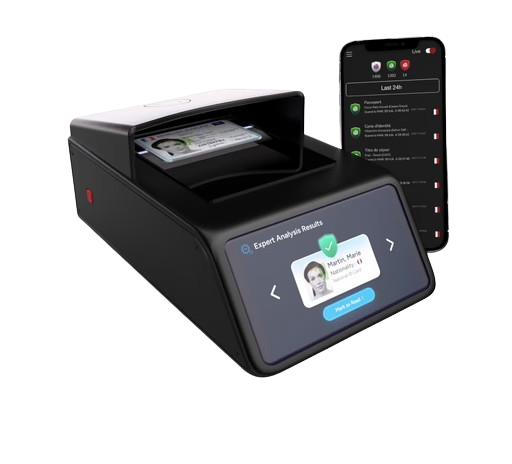
\includegraphics[width=.5\textwidth]{figures/Oneex desktop.png}
	      	\caption{\textit{Oneex Desktop}}
	      	\label{fig:Oneex desktop}
	      \end{figure}
	\item \textbf{Oneex Suitcase} : une valise mobile permettant de réaliser des contrôles sur le terrain , portable et robuste , elle laisse les utilisateurs se profiter d’un système mobile de vérification d’identité fiable et sécurisé.
	      \begin{figure}[ht]
	      	\centering
	      	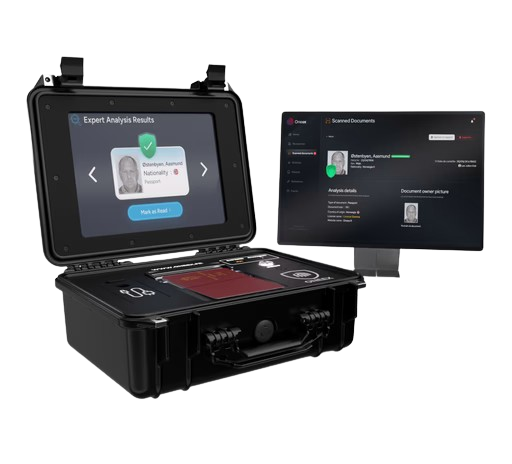
\includegraphics[width=.5\textwidth]{figures/Oneex suitcase.png}
	      	\caption{\textit{Oneex Suitcase}}
	      	\label{fig:Oneex Suitcase}
	      \end{figure}
	\item \textbf{Oneex Kiosk} : un kiosque en libre-service pour l’accueil et le contrôle des visiteurs. Permet Accueiller vos visiteurs sans assistance grâce à une vérification rapide et un accès direct.Une solution pensée pour vos opérations, combinant biométrie avancée et automatisation complète de l’accès visiteurs.
	      \begin{figure}[ht]
	      	\centering
	      	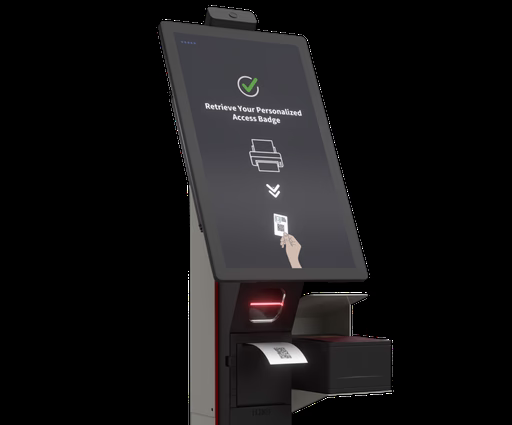
\includegraphics[width=.5\textwidth]{figures/Oneex kiosk.png}
	      	\caption{\textit{Oneex Kiosk}}
	      	\label{fig:Oneex Kiosk}
	      \end{figure}
\end{itemize}

Ces produits sont complétés par la suite logicielle Oneex Cloud et ScanApp, garantissant un pilotage centralisé et une intégration fluide dans les environnements clients.

\subsection{Services informatiques et outils internes}

Afin de garantir un haut niveau de qualité, Oneex s’appuie sur une infrastructure robuste et des outils modernes facilitant la gestion des opérations.

\subsubsection{Les services informatiques}

\textbf{Oneex ScanApp} constitue le cœur opérationnel de l’entreprise. Il assure l’analyse documentaire et la vérification d’identité, disponible sur postes fixes comme sur mobiles, avec une interface ergonomique et des fonctionnalités avancées. Il est constitué par une une interface utilisateur intuitive pour les ecrans des solutions que oneex offre et un moteur d’analyse de documents qui tourne localement , et est chargé par la lecture des documents , et l'execution d'une vingtaine d'algorithmes pour s'assurer de l'authenticité du document scanné. 

\textbf{Oneex Cloud} complète cet écosystème en permettant :

\begin{itemize}
	\item la gestion des vérifications,
	\item le suivi historique et la traçabilité,
	\item la sollicitation d’experts en cas de doute,
	\item l’analyse statistique des fraudes détectées.
\end{itemize}

\subsubsection{Les outils internes}

L’entreprise utilise plusieurs outils collaboratifs et techniques, parmi lesquels :
GitLab, Harbor, Nextcloud, Jitsi, Label Studio, YouTrack, Vault, SSO Keycloak.  
Les bases de données sont hébergées sur des serveurs dédiés et sécurisés, garantissant la confidentialité et la disponibilité des informations sensibles ainsi que la conformité aux réglementations et assurer un controle et une gestion des accès rigoureux.

\subsubsection{infrastructures internes}

Afin de garentir un controle total et une idependence aux fournisseurs de cloud, Oneex a opté pour une infrastructure IAAS (Infrastructure as a Service) hébergée dans des serveurs dont proxmox est installé et utilisé pour gerer toutes les ressources. Cette infrastructure est composée de serveurs physiques et virtuels, permettant de déployer les applications et services nécessaires à l’activité de l’entreprise.

\section{Les projets informatiques de la société}

\subsection{Introduction}

L’entreprise Oneex développe plusieurs projets informatiques stratégiques qui répondent à différents besoins métiers et techniques.

\subsection{Oneex Front}

Application frontend permettant la gestion des opérations, l’affichage des données et l’interaction avec les utilisateurs finaux.

\subsection{Oneex Back}

Backend exposant les API et orchestrant les processus métiers critiques.

\subsection{Oneex Scanner}

Solution logicielle dédiée à l’acquisition et à l’analyse des documents d’identité.

\subsection{Oneex ScanApp}

Application mobile ou desktop facilitant le scan et la vérification en temps réel des documents.

\subsection{Oneex CSharp}

Projet spécifique développé en C\# destiné à répondre à des besoins d’intégration ou d’outillage interne.

